\chapter{Model Evaluation}

We have observed the logistic model - foxes, birds, little things and all that. The voting schema looked reasonable. And before that, we have seen the model's predictions. They looked good. But how would we quantify the performance of the model?

\begin{wrapfigure}{o}{1.1\textwidth}
    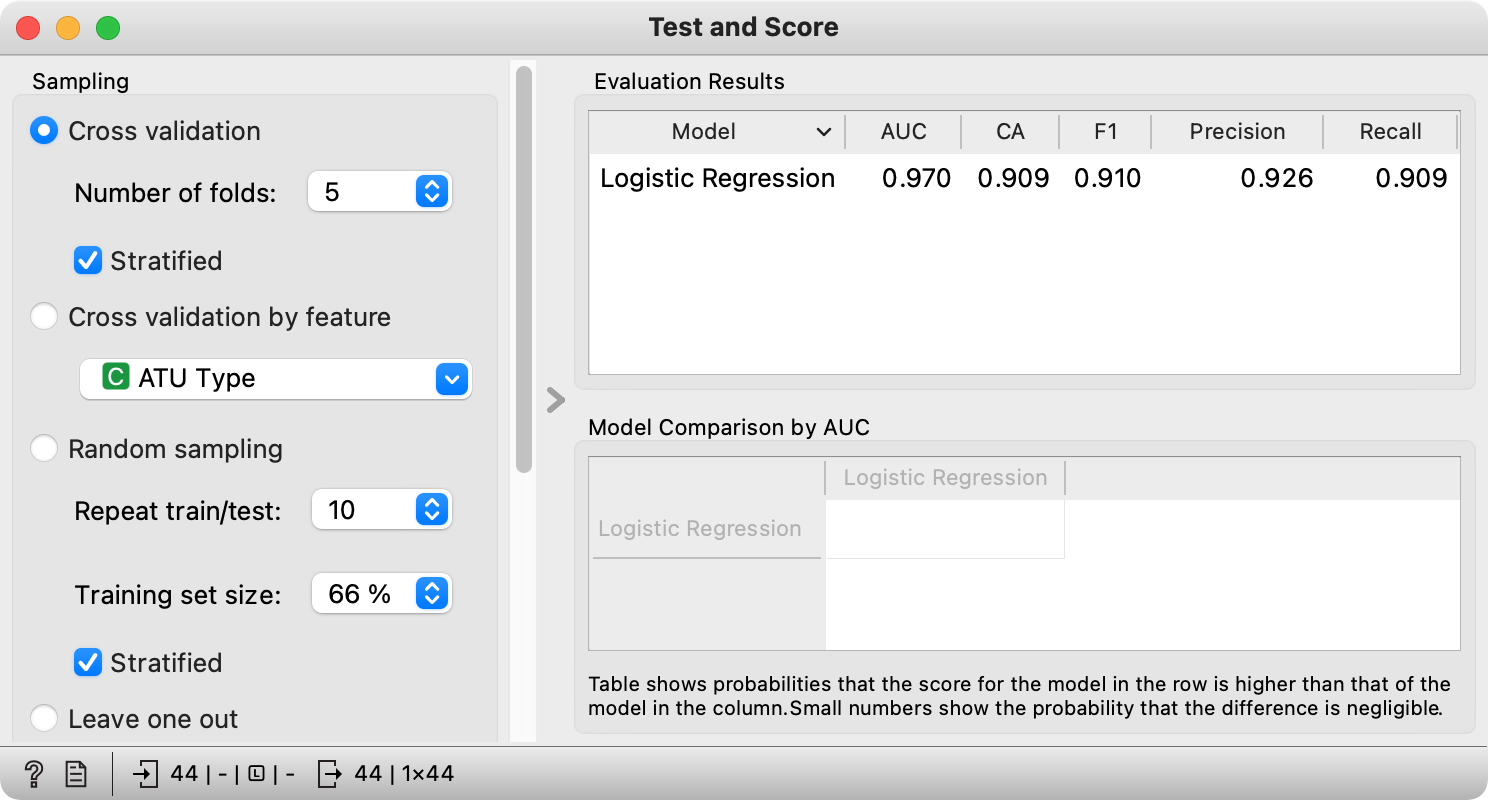
\includegraphics[scale=0.45]{test-and-score.png}
    \caption{$\;$}
\end{wrapfigure}

Perhaps we should just compute the proportion of the stories for which the model gave the correct answer? This score is called classification accuracy. For example, if we correctly predicted 40 tales out of 44, the classification accuracy would be 40/44 or 91\%.

AUC is another good measure to consider. In essence, the closer these two measures are to 1, the better the model's performance.

The widget that computes the classification accuracy is called \widget{Test and Score}. It needs two inputs: the data to test the model on and the modeling algorithm.\marginnote{\emph{It would make little sense asking whether Rapunzel is about animals after already telling the model that it is not.}\\
\\ 
Didn't we do this above in Predictions? Indeed, and this is why the predictions there were so excellent. Models should never be tested on the data from which they were constructed.}

\vspace{-0.2cm}
\begin{figure}[h]
  \centering
  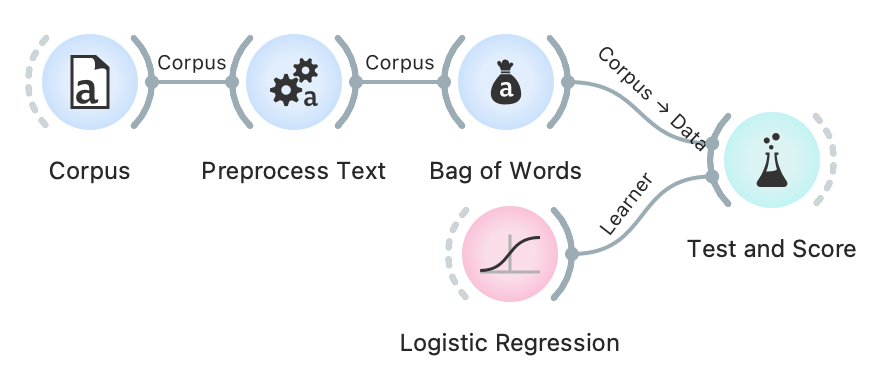
\includegraphics[width=\linewidth]{workflow.png}%
  \caption{$\;$}
\end{figure}
\vspace{-0.3cm}

This time, Logistic Regression doesn't need a data input. Instead, it provides a learner, which is a procedure for constructing the model. Test and Score then applies the learner multiple times on different data subsets. Each time, it constructs the model on a selected subset and uses the left-out data for testing. It would make little sense asking the model whether Rapunzel is an Animal Tale, after already telling it that it is not.
\clearpage
